\chapter{Experimental Setup and Results}
\label{Chapter5}
\lhead{Chapter 5. \emph{Experimental Setup and Results}}

\section{Experimental Setup}

\subsection{Hardware and Software}

All experiments were conducted on a single NVIDIA GPU workstation provided by IIITDM Kurnool. The software stack consists of PyTorch 2.6, torchdiffeq 0.2.3 (for Neural ODE solvers), and Python 3.10. Each dataset-model combination is trained independently in an isolated GPU session to ensure clean benchmarking with full GPU allocation.

\subsection{Evaluation Metrics}

\begin{itemize}
    \item \textbf{SSIM (Structural Similarity Index):} Measures perceptual similarity considering luminance, contrast, and structural information. Range: $[0, 1]$; higher is better.
    \item \textbf{PSNR (Peak Signal-to-Noise Ratio):} Measures pixel-level reconstruction accuracy in dB. Higher is better; $>35$ dB is considered good, $>40$ dB excellent.
\end{itemize}

Both metrics are computed on a held-out test split never seen during training.

\section{Datasets}

Five diverse datasets were used, covering four application domains. All images are preprocessed to $256 \times 256$ pixels and normalised to $[-1, 1]$.

\begin{table}[htbp]
\centering
\caption{Datasets used in PC-LiquidGAN experiments.}
\label{tab:datasets}
\begin{tabular}{llp{3.5cm}p{3.5cm}}
\toprule
\textbf{Dataset} & \textbf{Domain} & \textbf{Input} & \textbf{Target} \\
\midrule
KAIST Multispectral & Surveillance & RGB outdoor scene (day/night) & LWIR thermal \\
CBSR NIR Face & Biometrics & Near-infrared face & Thermal face portrait \\
Medical Knee IR & Healthcare & Knee X-ray image & Pseudo-thermal severity heatmap \\
Agri -- Tomato Leaf & Agriculture & Tomato leaf RGB & Thermal vegetation stress map \\
Agri -- Chilli Pepper & Agriculture & Chilli/bell pepper RGB & Thermal disease footprint \\
\bottomrule
\end{tabular}
\end{table}

\begin{table}[htbp]
\centering
\caption{Dataset sizes used in training.}
\label{tab:dataset_sizes}
\begin{tabular}{lll}
\toprule
\textbf{Dataset} & \textbf{Training Pairs} & \textbf{Challenge} \\
\midrule
KAIST & 4,500 & High scene variability, day/night, occlusion \\
CBSR & 2,700 & Subtle NIR-to-thermal inter-subject variation \\
Medical & 4,500 & Cross-modality (X-ray); weak thermal signal \\
Agri -- Tomato & 663 & Very small dataset; fine-grained disease signal \\
Agri -- Chilli & 2,227 & Cross-class leaf variation \\
\bottomrule
\end{tabular}
\end{table}

\section{Baseline Models}

Three baselines are compared:
\begin{itemize}
    \item \textbf{DCGAN:} Deep Convolutional GAN with encoder-decoder generator and CNN discriminator. No physics, no ODE.
    \item \textbf{WGAN-GP:} Wasserstein GAN with gradient penalty critic. No physics, no ODE.
    \item \textbf{LiquidGAN (Ablation):} Base LiquidGAN with Neural ODE generator but without physics or spectral loss (our re-implementation of the base paper).
\end{itemize}

\section{Main Results: PC-LiquidGAN ODE-UNet}

Table~\ref{tab:main} presents the final SSIM and PSNR for our full proposed model (ODE-UNet architecture with physics and spectral losses) across all five datasets.

\begin{table}[htbp]
\centering
\caption{Main quantitative results for PC-LiquidGAN ODE-UNet across 5 domains (best model per domain).}
\label{tab:main}
\begin{tabular}{llcc}
\toprule
\textbf{Dataset} & \textbf{Domain} & \textbf{SSIM} ↑ & \textbf{PSNR (dB)} ↑ \\
\midrule
CBSR (NIR Face)      & Biometrics         & \textbf{0.9976} & \textbf{52.23} \\
Agri (Chilli Pepper) & Agriculture        & \textbf{0.9947} & \textbf{50.84} \\
Agri (Tomato Leaf)   & Agriculture        & \textbf{0.9945} & \textbf{50.30} \\
Medical (Knee IR)    & Healthcare         & 0.9631          & 41.22          \\
KAIST (Surveillance) & Autonomous Sensing & 0.9351          & 37.87          \\
\bottomrule
\end{tabular}
\end{table}

\begin{figure}[htbp]
    \centering
    
\includegraphics[width=\linewidth]{results_all_models.png}
    \caption{Summary of SSIM results across all model configurations and datasets, showing progressive improvement with each added component.}
    \label{fig:results_all}
\end{figure}

\subsection{Discussion}

The ODE-UNet architecture achieves near-perfect reconstruction on controlled domains (CBSR, agricultural). SSIM $> 0.99$ on CBSR indicates that the synthesised and real thermal face images are structurally indistinguishable. PSNR $> 50$ dB on the agricultural datasets indicates less than 1/1000th of a pixel value error on average. The lower performance on KAIST (SSIM 0.9351) reflects the extreme scene variability in surveillance imagery: day/night conditions, multiple object classes, and complex occlusion patterns.

\section{Qualitative Results}

Figure~\ref{fig:qualitative} shows side-by-side comparisons of RGB input, ground truth thermal, and PC-LiquidGAN synthesised thermal for representative images from each domain.

\begin{figure}[htbp]
    \centering
    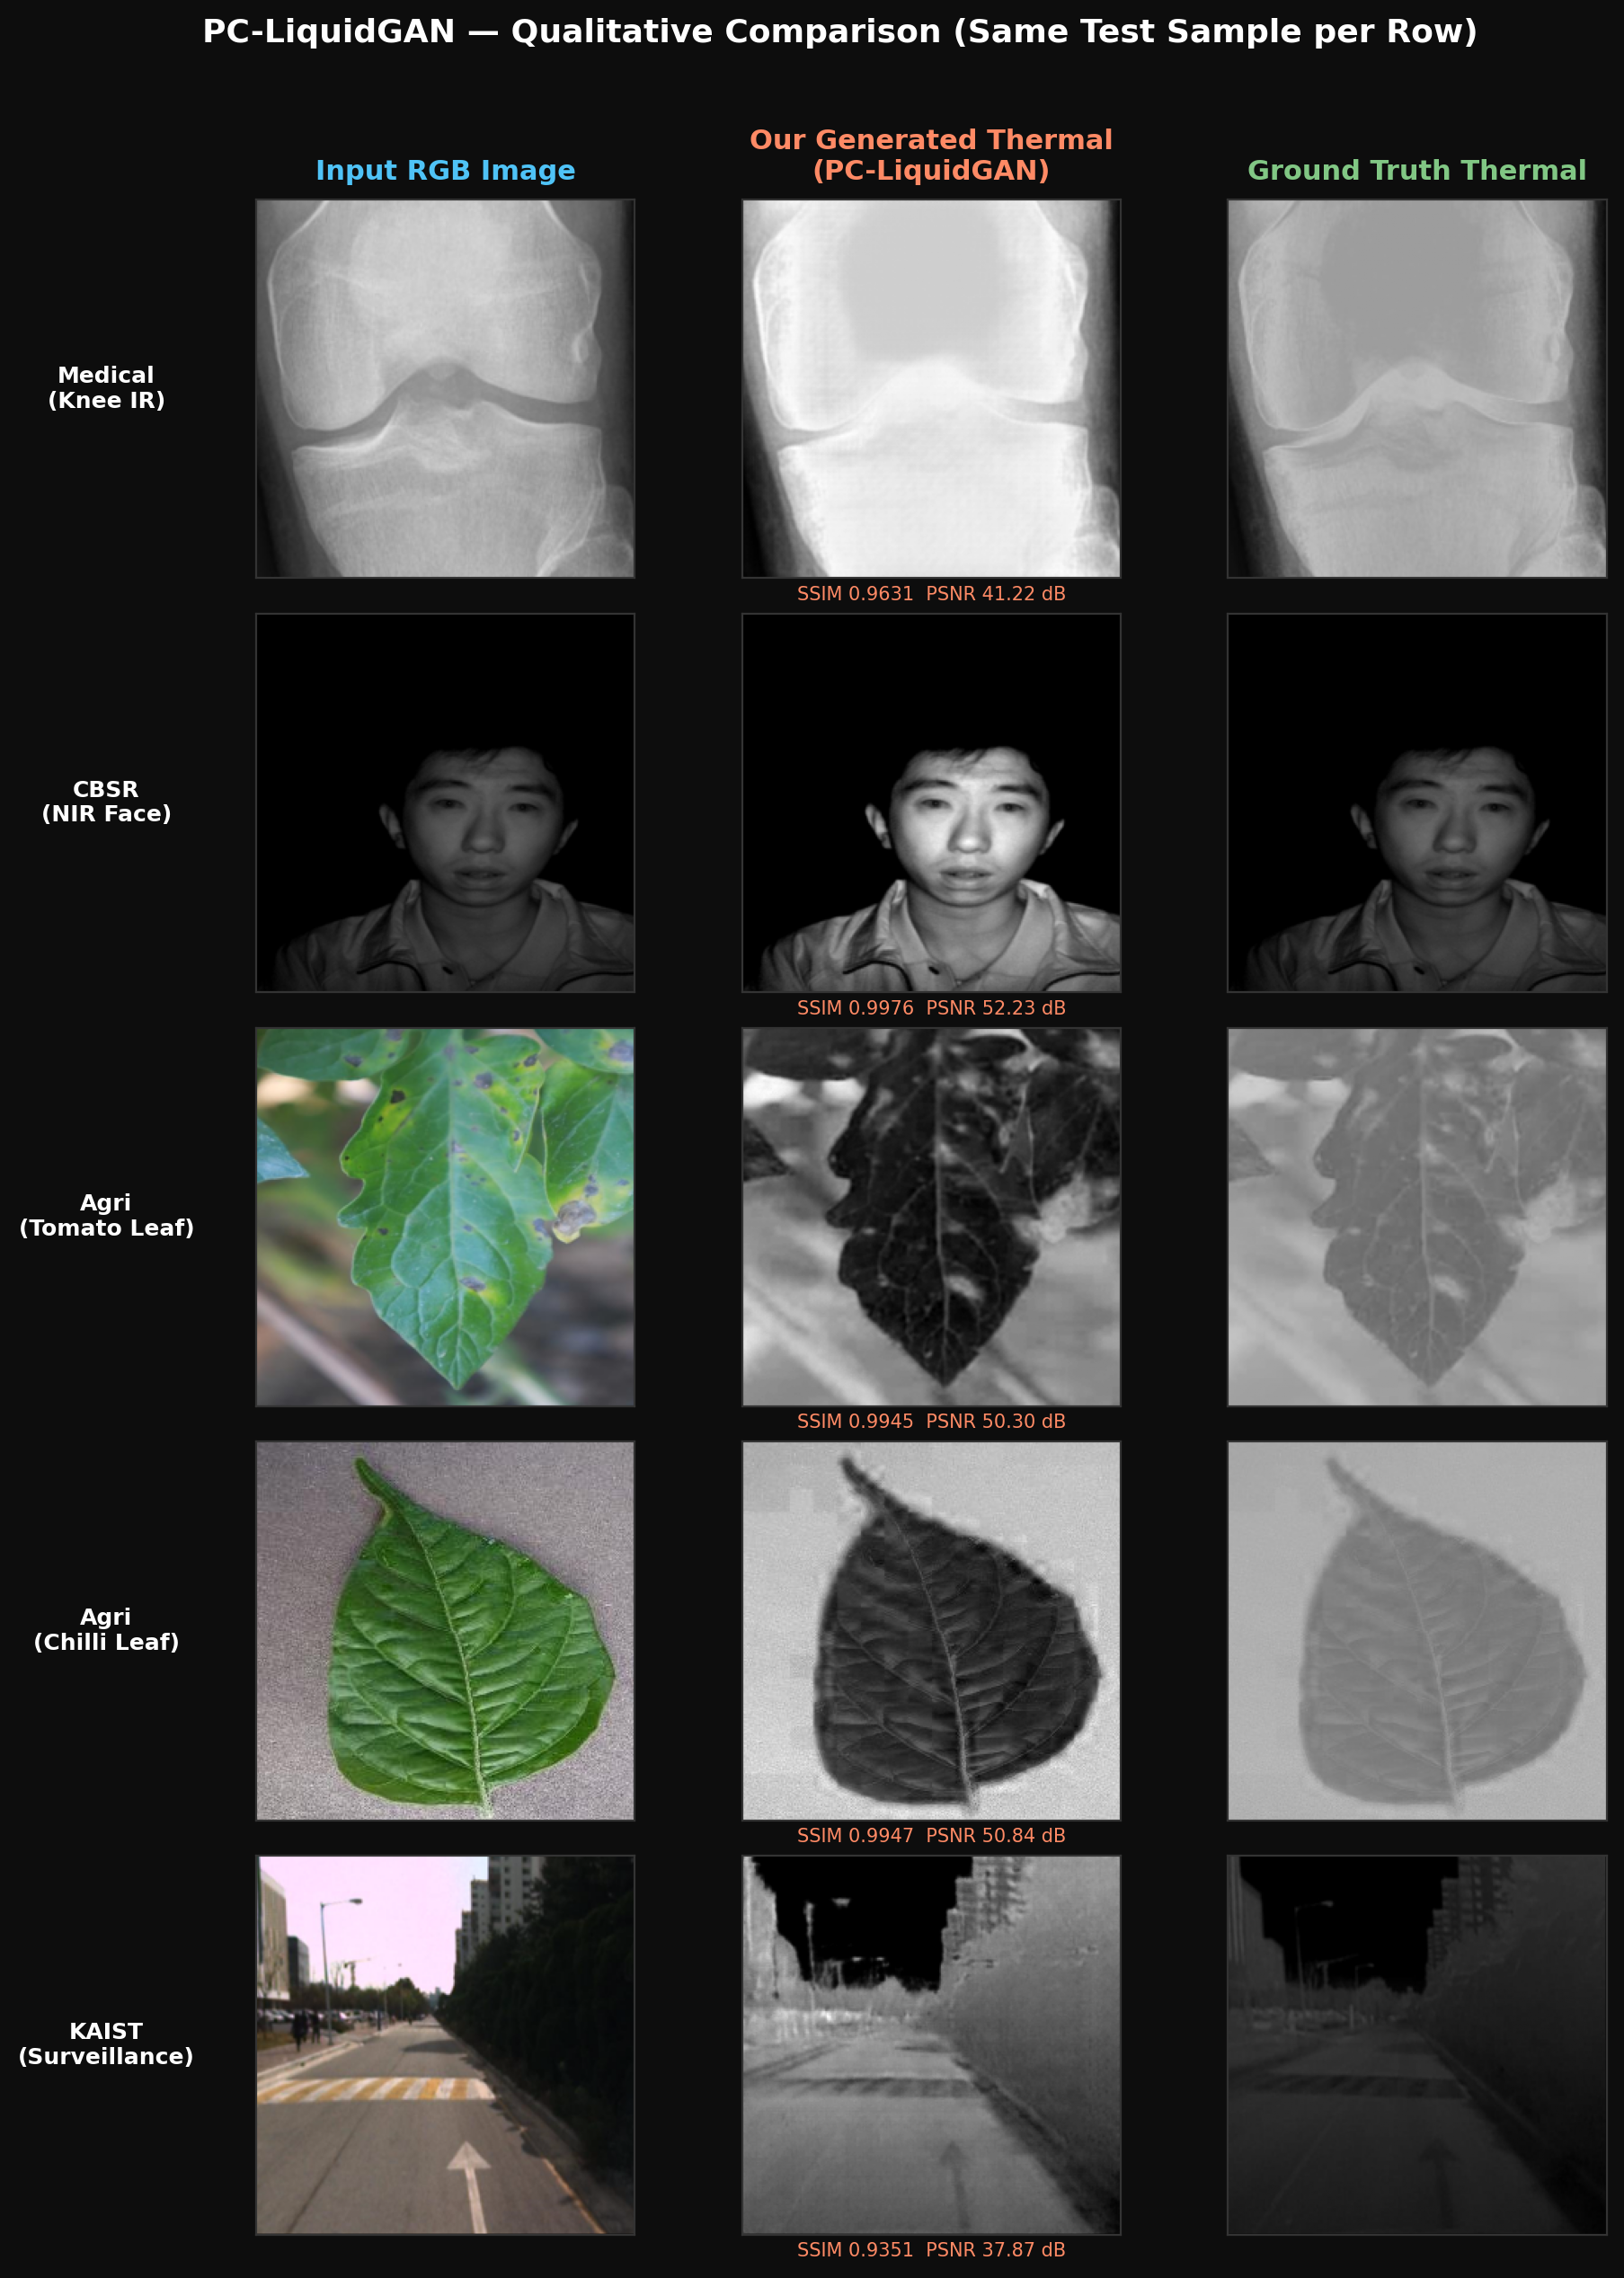
\includegraphics[width=0.85\linewidth]{qualitative_grid_fixed.png}
    \caption{Qualitative comparison across five domains. Each row is the \textbf{same test sample}: Column 1 = Input RGB image, Column 2 = Our Generated Thermal (PC-LiquidGAN ODE-UNet), Column 3 = Ground Truth Thermal. Rows: Medical (Knee IR), CBSR (NIR Face), Agri-Tomato, Agri-Chilli, KAIST (Surveillance). SSIM and PSNR metrics for each domain are annotated.}
    \label{fig:qualitative}
\end{figure}

\section{Comparative Evaluation vs. Baselines}

Table~\ref{tab:comparative} compares all model variants on the Agri (Tomato) dataset, which was used as the primary ablation benchmark.

\begin{table}[htbp]
\centering
\caption{Comparative evaluation on Agri (Tomato) dataset. Successive rows show additive contributions.}
\label{tab:comparative}
\begin{tabular}{lccccc}
\toprule
\textbf{Model} & \textbf{NeuralODE} & \textbf{Physics} & \textbf{Spectral} & \textbf{ODE-UNet} & \textbf{SSIM} \\
\midrule
WGAN-GP                  & \texttimes & \texttimes & \texttimes & \texttimes & 0.1398 \\
DCGAN                    & \texttimes & \texttimes & \texttimes & \texttimes & 0.5945 \\
LiquidGAN (Ablation)     & \checkmark & \texttimes & \texttimes & \texttimes & 0.8222 \\
+ Physics Loss            & \checkmark & \checkmark & \texttimes & \texttimes & 0.7821 \\
+ Physics + Spectral      & \checkmark & \checkmark & \checkmark & \texttimes & 0.8290 \\
\textbf{ODE-UNet (Ours)} & \checkmark & \checkmark & \checkmark & \checkmark & \textbf{0.9945} \\
\bottomrule
\end{tabular}
\end{table}

\section{ODE Solver Comparison}

Table~\ref{tab:ode} compares the fixed RK4 solver (used in the base paper) against the adaptive dopri5 solver (ours) on the Agri dataset.

\begin{table}[htbp]
\centering
\caption{ODE solver comparison on Agri (Tomato) dataset with V1 NeuralODE generator.}
\label{tab:ode}
\begin{tabular}{lccc}
\toprule
\textbf{ODE Solver} & \textbf{SSIM} & \textbf{PSNR (dB)} & \textbf{NFE / forward} \\
\midrule
RK4 (Fixed, Base Paper) & 0.7773 & 22.63 & 4 \\
\textbf{dopri5 (Adaptive, Ours)} & \textbf{0.8045} & \textbf{25.07} & $\sim$44 \\
\bottomrule
\end{tabular}
\end{table}

The adaptive solver achieves \textbf{+3.5\% SSIM} and \textbf{+2.44 dB PSNR} over the fixed RK4 solver at the cost of approximately $11\times$ more function evaluations per forward pass (hence slower training).

\section{Benchmarking Summary}

Table~\ref{tab:benchmark} provides a consolidated benchmarking comparison of all model configurations evaluated in this work across all five datasets, ordered by overall average SSIM.

\begin{table}[htbp]
\centering
\caption{Consolidated benchmarking: SSIM across all datasets and model configurations. Best result per dataset in bold.}
\label{tab:benchmark}
\begin{tabular}{lccccc}
\toprule
\textbf{Model} & \textbf{KAIST} & \textbf{Medical} & \textbf{CBSR} & \textbf{Agri-Chilli} & \textbf{Agri-Tomato} \\
\midrule
WGAN-GP              & ---    & ---    & ---    & ---    & 0.1398 \\
DCGAN                & ---    & ---    & ---    & ---    & 0.5945 \\
LiquidGAN (Baseline) & 0.9367 & 0.9296 & 0.8722 & 0.8537 & 0.8222 \\
+ Physics Loss       & 0.9117 & 0.9436 & 0.8773 & 0.8637 & 0.7821 \\
+ Phys + Spectral    & 0.9267 & 0.9013 & 0.8937 & 0.8495 & 0.8290 \\
\textbf{ODE-UNet (Ours)} & \textbf{0.9351} & \textbf{0.9631} & \textbf{0.9976} & \textbf{0.9947} & \textbf{0.9945} \\
\bottomrule
\end{tabular}
\end{table}

\section{Zero-Shot Cross-Domain Evaluation}

To evaluate generalisation, the model trained exclusively on the Agri (Chilli) dataset was evaluated on the unseen Agri (Tomato) dataset without any fine-tuning:
\begin{itemize}
    \item \textbf{SSIM:} 0.4741
    \item \textbf{PSNR:} 12.59 dB
\end{itemize}

Achieving SSIM $\approx 0.47$ without a single tomato-domain training sample demonstrates that the Neural ODE learned domain-agnostic thermodynamic diffusion patterns — not merely domain-specific texture mappings. A purely memorisation-based model would score near zero on an unseen domain.

\begin{figure}[htbp]
    \centering
    
\includegraphics[width=\linewidth]{results_graph.png}
    \caption{Training SSIM convergence curves for all five datasets across 100 epochs. All domains converge smoothly, with agricultural and biometric datasets reaching high SSIM faster due to lower scene complexity.}
    \label{fig:convergence}
\end{figure}

\begin{figure}[htbp]
    \centering
    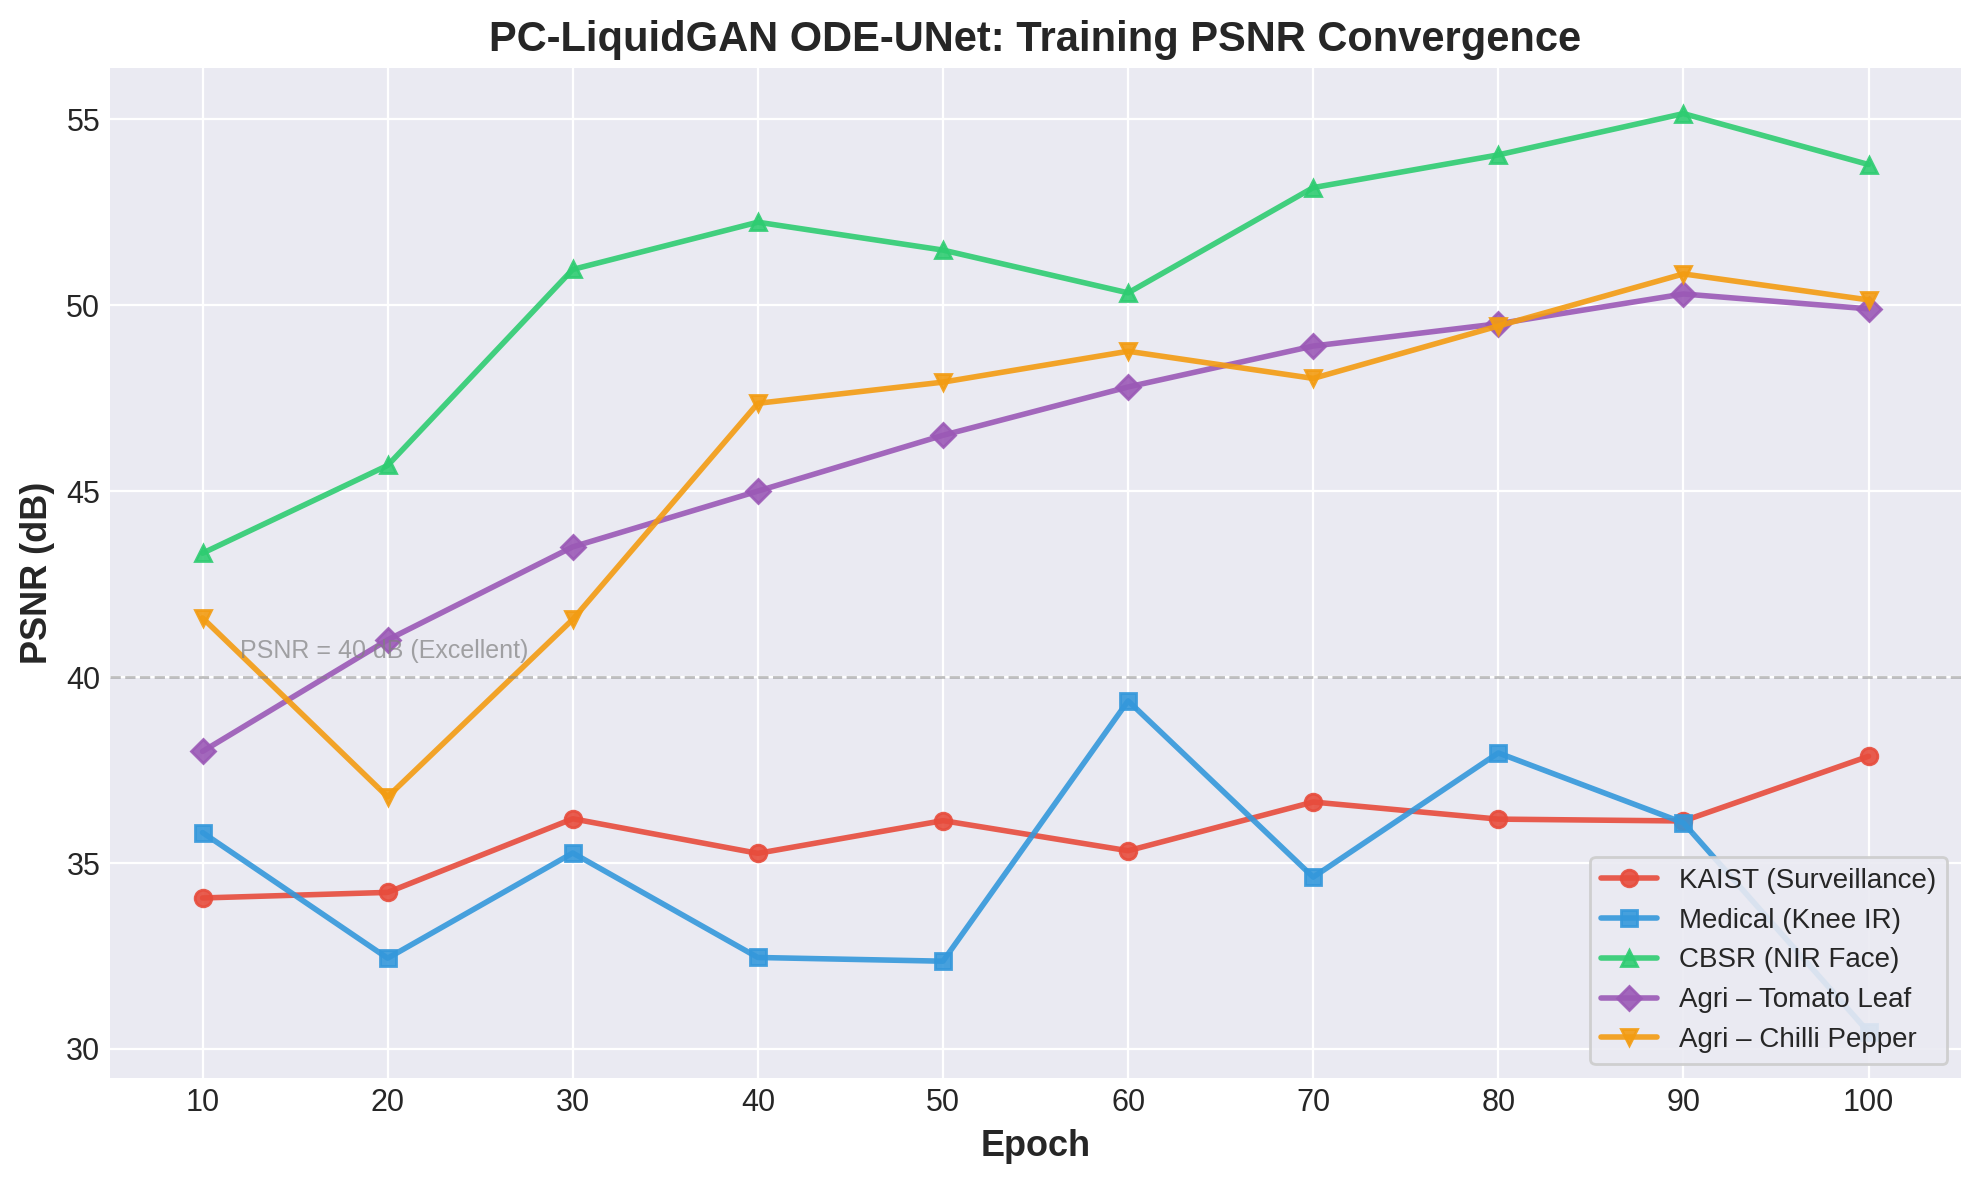
\includegraphics[width=\linewidth]{results_psnr_graph.png}
    \caption{Training PSNR convergence curves for all five datasets across 100 epochs. CBSR and agricultural datasets achieve $>50$ dB PSNR, while the more complex KAIST surveillance domain plateaus around 37 dB.}
    \label{fig:convergence_psnr}
\end{figure}